% Modelo de monografia criado para a Faculdade de Computação
% da Universidade Federal do Pará a partir da classe abntex2.
% Este documento só deverá ser alterado para incluir ou excluir
% elementos pré e pós textuais. Use o comentário do latex (%) caso
% deseje excluir algum elemento.

%% abtex2-modelo-trabalho-academico.tex, v-1.9.6 laurocesar
%% Copyright 2012-2016 by abnTeX2 group at http://www.abntex.net.br/
%%
%% This work may be distributed and/or modified under the
%% conditions of the LaTeX Project Public License, either version 1.3
%% of this license or (at your option) any later version.
%% The latest version of this license is in
%%   http://www.latex-project.org/lppl.txt
%% and version 1.3 or later is part of all distributions of LaTeX
%% version 2005/12/01 or later.
%%
%% This work has the LPPL maintenance status `maintained'.
%%
%% The Current Maintainer of this work is the abnTeX2 team, led
%% by Lauro César Araujo. Further information are available on
%% http://www.abntex.net.br/
%%
%% This work consists of the files abntex2-modelo-trabalho-academico.tex,
%% abntex2-modelo-include-comandos and abntex2-modelo-references.bib
%%

% ------------------------------------------------------------------------
% ------------------------------------------------------------------------
% abnTeX2: Modelo de Trabalho Academico (tese de doutorado, dissertacao de
% mestrado e trabalhos monograficos em geral) em conformidade com
% ABNT NBR 14724:2011: Informacao e documentacao - Trabalhos academicos -
% Apresentacao
% ------------------------------------------------------------------------
% ------------------------------------------------------------------------

\documentclass[
	% -- opções da classe memoir --
	12pt,				% tamanho da fonte
	openright,			% capítulos começam em pág ímpar (insere página vazia caso preciso)
	oneside,			% para impressão em frente e verso. Oposto a oneside
	a4paper,			% tamanho do papel.
	% -- opções da classe abntex2 --
	chapter=TITLE,		% títulos de capítulos convertidos em letras maiúsculas
	%section=TITLE,		% títulos de seções convertidos em letras maiúsculas
	%subsection=TITLE,	% títulos de subseções convertidos em letras maiúsculas
	%subsubsection=TITLE,% títulos de subsubseções convertidos em letras maiúsculas
	% -- opções do pacote babel --
	english,			% idioma adicional para hifenização
	french,				% idioma adicional para hifenização
	spanish,			% idioma adicional para hifenização
	brazil				% o último idioma é o principal do documento
	]{abntex2}

% ---
% Pacotes básicos
% ---
\usepackage{lmodern}			% Usa a fonte Latin Modern
\usepackage{mathptmx}			% Usa a fonte Times New Roman
\usepackage[T1]{fontenc}		% Selecao de codigos de fonte.
\usepackage[utf8]{inputenc}		% Codificacao do documento (conversão automática dos acentos)
\usepackage{lastpage}			% Usado pela Ficha catalográfica
\usepackage{indentfirst}		% Indenta o primeiro parágrafo de cada seção.
\usepackage{color}				% Controle das cores
\usepackage{graphicx}			% Inclusão de gráficos
\usepackage{subcaption}				% Inclusão de gráficos lado a lado
\usepackage{microtype} 			% para melhorias de justificação
\usepackage{tabularx,ragged2e}	% Para inserir tabelas
\usepackage{multirow}			% Para mesclar células
\usepackage[dvipsnames,table,xcdraw]{xcolor}		% Permite adicionar cores nas linhas de tabelas
\usepackage{fancyvrb}			% Permite adicionar arquivos de texto
\usepackage[portuguese, ruled, linesnumbered]{algorithm2e} % Uso de algoritmos
\usepackage{amsfonts}			% Permite usar notação de conjuntos
\usepackage{amsmath}			% Permite citar equações
\usepackage{amsthm}				% Permite criar teoremas e experimentos
\usepackage[font={bf, small}, labelsep=endash, labelfont=bf]{caption}	% Faz legenda de figuras ficarem em negrito
\usepackage{cancel}				% Permite fazer expressão tendendo a zero
\usepackage{graphicx,import}

\usepackage{epstopdf}			% Converte eps para pdf
\usepackage[final]{pdfpages}

\newcolumntype{L}{>{\RaggedRight\arraybackslash}X}
% ---

% ---
% Pacotes adicionais, usados apenas no âmbito do Modelo Canônico do abnteX2
% ---
\usepackage{lipsum}				% para geração de dummy text
% ---

% ---
% Pacotes de citações
% ---
%\usepackage[brazilian,hyperpageref]{backref}	 % Paginas com as citações na bibl
\usepackage[alf, abnt-emphasize=bf]{abntex2cite}	% Citações padrão ABNT

% ---
% Customizações para o layout da UFPA
% ---
\usepackage{modelo-ufpa/ufpa}

% Muda o título de lista de ilustrações para lista de figuras
\addto\captionsbrazil{%
  \renewcommand{\listfigurename}%
    {Lista de Ilustrações}%
	\renewcommand{\listtablename}%
    {Lista de Tabelas}%
}

% Permite utilizar figuras sem precisar colocar o caminho absoluto
\graphicspath{{imagens/}}

% Define o ambiente de experimentos
\theoremstyle{definition}
\newtheorem{experimento}{Experimento}[section]
\newcommand{\experimentoautorefname}{Experimento}

% ---
% CONFIGURAÇÕES DE PACOTES
% ---

% ---
% Configurações do pacote backref
% Usado sem a opção hyperpageref de backref
%\renewcommand{\backrefpagesname}{Citado na(s) página(s):~}
% Texto padrão antes do número das páginas
%\renewcommand{\backref}{}
% Define os textos da citação
%\renewcommand*{\backrefalt}[4]{
%	\ifcase #1 %
%		Nenhuma citação no texto.%
%	\or
%		Citado na página #2.%
%	\else
%		Citado #1 vezes nas páginas #2.%
%	\fi}%
% ---

% ---
% Informações de dados para CAPA, FOLHA DE ROSTO e FICHA CATALOGRÁFICA
% ---
\universidade{UNIVERSIDADE FEDERAL DO PARÁ}
\instituto{INSTITUTO DE TECNOLOGIA - ITEC}
\faculdade{Programa de pós graduação em engenharia eltétrica}
\titulo{Transformer networks aplicada a reconhecimento automatico de voz}
\autor{Rodrigo Gomes Dutra}

\local{Belém}
\data{2021}

% ---
% Configurações de aparência do PDF final

% alterando o aspecto da cor azul
\definecolor{blue}{RGB}{41,5,195}

% informações do PDF
\makeatletter
\hypersetup{
     	%pagebackref=true,
		pdftitle={\imprimirtitulo},
		pdfauthor={\imprimirautor},
    	pdfsubject={\imprimirpreambulo},
	    pdfcreator={LaTeX with abnTeX2},
		pdfkeywords={\imprimirpalavraschave},
		colorlinks=true,       		% false: boxed links; true: colored links
    	linkcolor=black,          	% color of internal links
    	citecolor=black,        		% color of links to bibliography
    	filecolor=magenta,      		% color of file links
		urlcolor=blue,
		bookmarksdepth=4,
        breaklinks=true
}
\makeatother
% ---

% ---
% Espaçamentos entre linhas e parágrafos
% ---

% O tamanho do parágrafo é dado por:
\setlength{\parindent}{1.3cm}

% Controle do espaçamento entre um parágrafo e outro:
\setlength{\parskip}{0.2cm}  % tente também \onelineskip

% ---
% compila o indice
% ---
\makeindex
% ---

% ----
% Início do documento
% ----
\begin{document}

% Seleciona o idioma do documento (conforme pacotes do babel)
%\selectlanguage{english}
\selectlanguage{brazil}

% Retira espaço extra obsoleto entre as frases.
\frenchspacing

% ----------------------------------------------------------
% ELEMENTOS PRÉ-TEXTUAIS
% ----------------------------------------------------------
% \pretextual

% ---
% Capa
% ---
\imprimircapa
% ---

% ----------------------------------------------------------
% ELEMENTOS TEXTUAIS
% ----------------------------------------------------------
\textual

% ----------------------------------------------------------
% Introdução
% ----------------------------------------------------------
\chapter{Introdução}
\label{cap:introducao}
Este trabalho busca demonstrar o uso preliminar de redes neurais do tipo transformer networks \citeonline{vaswani2017attention} aplicada na tarefa de reconhecimento automático de voz. Nesse sentido a tarefa consiste em classificar palavras isoladas retiradas do banco de dados speach commands \citeonline{warden2018speech}, para isso foi utilizado o programa spock \citeonline{Ak2021},para pre-processar os sinais de voz em formato WAV, extraindo assim features acústicas utilizando a técnica de Mel-frequency cepstral coefficients (MFCC). Após a extração das features acústicas o modelo então é treinado para a classificação da classe da palavra dado a entrada de features acústica fornecida

Para a tarefa em questão de reconhecimento automático de voz, atualmente as redes neurais do tipo recorrente (RNNS) e long short term memory (LSTM), representam o estado da arte \citeonline{zeng2021semi}, juntamente com redes convolucionais. Entretanto, redes neurais do tipo transformers ultrapassam redes neurais do tipo recorrentes em aplicações de processamento de linguagem natural[] e predição de séries temporais, dessa forma apresentam grande potencial para alcançar resultados promissores na área de reconhecimento automatico de voz.

A fim de comparar o resultado do modelo, o programa spock utiliza a técnica de hmm, assim esta será utilizado como baseline. Ambas as tecnicas serão treinadas para reconhecer as seguintes palavras: dog, cat, house, happy e zero. Para a composição do dataset de treino foi escolhido cem audios em formato wav para cada palavra e para teste serão utilizados vinte e cinco audios de cada palavra.


% ---
% Capitulo com exemplos de comandos inseridos de arquivo externo
% ---
\include{abntex2-modelo-include-comandos}
% ---

% ----------------------------------------------------------
% Referenciais Teóricos
% ----------------------------------------------------------
\chapter{Desenvolvimento}
\label{cap:referenciais_teoricos}

\section{Pre-processamento de dados}
Reconhecimento automático de voz de palavras isoladas é uma tarefa de aprendizado supervisionado, de forma que o audio é a entrada do modelo e a saída do modelo é a classe da palavra  correspondente ao audio de entrada. Dessa forma a fim de reduzir o ruído do sinal de entrada e extrair as features acústicas do sinal é aplicado a técnica de MFCC.

Assim o esquemático do MFCC é como segue:

\begin{itemize}
	\item Janelamento do sinal
	\item Transformada de fourier discreta (DFT)
	\item Mel-filter Bank
	\item Conversão para escala logarítmica
	\item Transformada inversa
\end{itemize}

A etapa de janelamento do sinal consiste em retirar segmentos do sinal, no caso da implementação de 240ms, para posteriormente ser processado e retirado as features acústicas de cada segmento.

A partir desse ponto o sinal então passa pela transformada discreta de fourier, dado que esse sinal de entrada é um audio em formato WAV e trata-se de um sinal digital. Dessa forma é obtido o sinal no domínio da frequência, onde é este pode ser analisado de maneira mais simples.

O Mel-filter bank consiste em um método de imitar a percepção humana do som para as maquinas. O ouvido humano tem uma percepção diferente para diferentes frequências, ao passo que nas maquinas as frequências tem a mesma resolução, então são percebidas da mesma forma. Dessa forma esse método realiza o mapeamento abaixo:

\begin{align}
	mel(f) = 1127ln(1+ \frac{1}{700})
\end{align}

Após esse passo  é realizado a conversão para escala logarítmica e então é realizado a transformada de fourrier inversa para o dominio do tempo. Nesse passo o algoritimo seleciona os primeiros 12 coeficientes do sinal antes de realizar a transformada inversa. Juntamente com os 12 coeficientes, também é retirado a energia do sinal como uma feature. Juntamente com as 13 features retiradas também é realizado a primeira e a segunda derivada dessas 13 features iniciais, gerando mais 26 features,  e o total de 39 features por segmento do sinal inicial.

\section{Transformer networks}
As transformer networks foram construidas pelo autor \citeonline{vaswani2017attention} para processar dados sequenciais e potencialmente ultrapassar a performance das redes neurais do tipo LSTM para a tarefa de processamento de linguagem natural. Após essa aplicação muitas outras surgiram fora do campo de processamento de linguagem natural, como em séries temporais \citeonline{wu2020deep} \citeonline{zhou2021informer} e até mesmo para classificação de imagens \citeonline{chen2021crossvit}. Em todas essas aplicações o modelo baseado em transformer networks consegue ultrapassar os modelos estado da arte tanto em performance quanto em custo computacional, além do fato de possibilitar processamento paralelo entre várias maquinas, tarefa a qual não pode ser efetuada quando utilizado modelos baseados em redes recorrentes.

No contexto de reconhecimento automático de voz, a rede do tipo transformers também foi capaz de atingir performance maior que os modelos considerados estado da arte \citeonline{lu2020exploring}. Dessa forma é um modelo interessante para se avaliar nesse contexto, de forma prática.

Portanto, foi utilizado o somente o encoder da arquitetura encoder decoder da rede transformer, como mostrado abaixo:

\begin{figure}[!htb]
	\caption{Estrutura do transformer encoder}
	\label{fig:estrutura_dna}
	\centering
	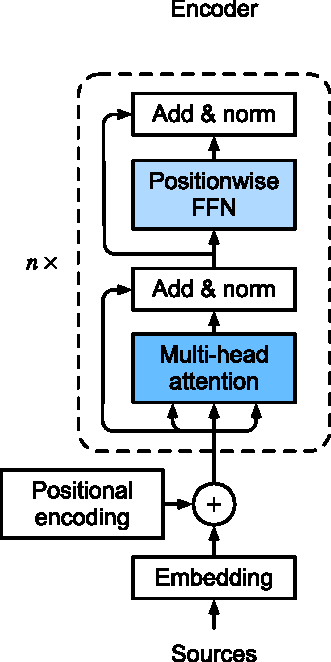
\includegraphics[width=4cm]{transformer_encoder.pdf} \\
	\begin{small}\textbf{Fonte: O Autor (2021)}\end{small}
\end{figure}

O encoder do transformer utiliza como entrada uma matriz de três dimensões: batch, passo de tempo, features. No caso desse trabalho essa estrutura irá ficar da forma batch, segmento, features acústicas.

Diferentemente de redes neurais recorrentes, como a LSTM, a transformer network utiliza do positional encoding para adicionar a noção de ordem temporal no modelo. O positional encoding faz isso por meio de senos e cossenos de diferentes frequencias, inserindo assim a noção de sequencia na matriz de entrada

\begin{align}
	PE_{pos, 2i} = sin(pos/1000^{2i/d_{model}}), \\
	PE_{pos, 2i+1} = cos(pos/1000^{2i/d_{model}}),
	\label{eq:pe}
\end{align}

Após o processo do positional encoding a entrada passa pelo processo do encoder, onde o tensor agora irá passar pelo processo das multiplas attention heads, onde é gerado uma matriz de self attention. Essa matriz de self attention é o mecanismo que a rede transformer utiliza para focar nos pontos mais importantes da sequencia de entrada. Depois desse processo é efetuado normalizações e outras operações por camadas do tipo feed forward.

Após o processo do encoder, a informação é passada por uma camada simples do tipo feed forward para realizar a classificação da palavra isolada. A imagem abaixo retrata o fluxo do modelo total de forma simples:

\begin{figure}[!htb]
	\caption{Estrutura do modelo transformer}
	\label{fig:trans_pipe}
	\centering
	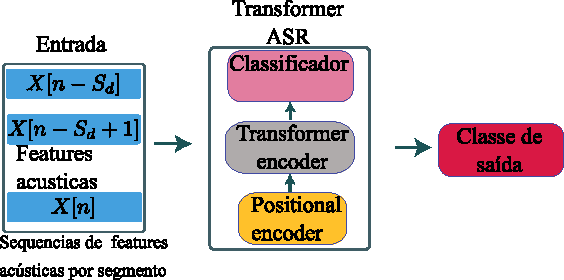
\includegraphics{transformer.pdf} \\
	\begin{small}\textbf{Fonte: O Autor (2021)}\end{small}
\end{figure}

Onde, na figura \ref{fig:trans_pipe} cada vetor $X[n]$ contem as 39 features acústicas, e a entrada total é uma matriz composta por 197 vetores de features acústicas. A implementação completa pode ser acessada em: \citeonline{Rd2021}.

\newpage
% ---
\section{Baseline}
% ---

O baseline trata-se do algoritmo que utiliza de hidden markov models (HMMs) para realizar a classificação, dado  as features acústicas de entrada. HMMs são modelos estatísticos que podem ser utilizados na área de aprendizado de máquina, para tarefas de classificação. O objetivo desse modelo é aprender a tarefa como uma cadeia de markov, por observar os estados escondidos.

A fim de implementação, o baseline composto por 5 HMMs, com o número de gaussianas variando de 1 a 5, foi executado pelo programa spock \citeonline{Ak2021} em forma de guided user interface (GUI) para o processamento dos arquivos WAV em features acústicas e posteriormente para a tarefa de reconhecimento automático de voz utilizando as HMMS.


\chapter{Experimento e resultados}
\label{cap:implementacao}
Os modelos foram postos a prova utilizando o dataset speach commands \citeonline{warden2018speech}, segmentando o dataset para conter somente as palavras : dog, cat, house, happy e zero, com 100 amostras sonoras para cada palavra no dataset de treinamento e 25 amostras sonoras de cada palavra para teste.

Após a seleção do dataset, foi executado o programa spock para o pre-processamento dos dados para o modelo baseado em transformer networks e para geração do baseline. Com os audios de entrada ja processados em features acústicas por segmentos, é então iniciado o passo de normalização para utilizar essas features como entrada no modelo transformer.

Depois da normalização, os dados são formatados a fim de entrar uma matriz com dimensões iguais a batch, segmento, features acústicas para o modelo, de forma que o modelo transformer irá traçar a relação entre cada passo de tempo (segmento) utilizando o mecanismo de self attention e a partir disso irá fazer a inferência de classificação.
Abaixo segue o erro e a acurácia por época. Onde para a validação do modelo foi utilizado 25 exemplos de audio para cada palavra.

\begin{figure}[!h]
	\caption{Erro por época}
	\label{fig:trans_pipe}
	\centering
	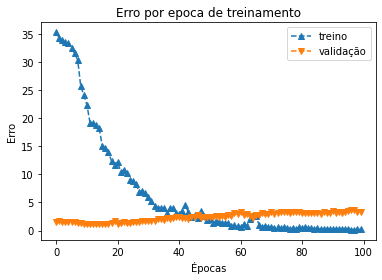
\includegraphics[width=10cm]{loss.png} \\
	\begin{small}\textbf{Fonte: O Autor (2021)}\end{small}
\end{figure}

Após o treinamento, o modelo pode realizar a classificação com $72\%$ de acurácia total, demonstrando valores diferentes de acertividade de acordo com a palavra. Como mostrado na matriz de confusão na figura \ref{fig:mtr}.

\begin{figure}[!h]
	\caption{Acurácia por época}
	\label{fig:trans_pipe}
	\centering
	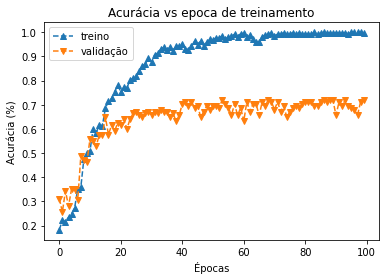
\includegraphics[width=10cm]{acc.png} \\
	\begin{small}\textbf{Fonte: O Autor (2021)}\end{small}
\end{figure}

\begin{figure}[!h]
	\caption{Matriz de confusão}
	\label{fig:mtr}
	\centering
	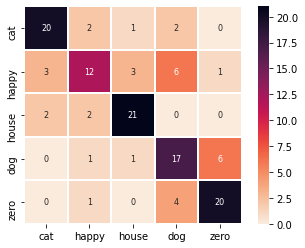
\includegraphics{mtr.png} \\
	\begin{small}\textbf{Fonte: O Autor (2021)}\end{small}
\end{figure}

\newpage
Agora comparando-se com o baseline composto por HMMs, temos na tabela \ref{tab:modelos}, que o modelo composto pela rede neural do tipo transformers foi capaz de ultrapassar somente o modelo baseado em HMM que é formado utilizando somente uma gaussiana. Outro fato interessante é que ao aumentar a complexidade dos modelos HMM estes começam a perder performance, o que indica que os modelos podem ter caído no estado de overfitting.
\begin{quadro}[!h]
	\centering
	\caption{Comparação dos modelos}
	\label{tab:modelos}
	\begin{tabular}{lccc}
		\toprule
		\multicolumn{1}{c}{\textbf{Modelo}} & \textbf{\textit{Acurácia total}} \\ \midrule

		Transformer network                 & $72.0\%$                         \\

		HMMs  com $1$ gaussianas            & 66.4\%                           \\

		HMMs  com $2$ gaussianas            & 72.8\%                           \\

		HMMs  com $3$ gaussianas            & 79.2\%                           \\
		HMMs  com $4$ gaussianas            & 78.4\%                           \\

		HMMs  com $5$ gaussianas            & 76.8\%                           \\
		\bottomrule                                                            \\
	\end{tabular}
\end{quadro}


% ----------------------------------------------------------
% Resultados e Discussão
% ----------------------------------------------------------


% ----------------------------------------------------------
% Considerações Finais
% ----------------------------------------------------------
\chapter{Conclusão}
\label{conclusao}

De posse dos resultados é possível notar uma quebra de expectativa entre a escolha de um modelo que está sendo altamente utilizado para vários problemas com dados sequenciais e um modelo consolidado estatístico probabilístico. De modo que o modelo baseado em transformer networks não ultrapassou a performance do melhor modelo baseado em HMMs como o esperado ao ler trabalhos que retratam o estado da arte do campo de reconhecimento automático de voz utilizando palavras isoladas.

Uma razão para tal resultado é pelo fato de redes neurais complexas precisarem de uma base de dado extensa e representativa para poderem generalizar melhor. Dessa forma talvez a escolha de 100 amostras de audio por palavra pode não ter ajudado a rede transformer a alcançar seu potencial máximo. Ao passo disso é importante notar a relevancia de modelos consolidados na literatura, de forma que mesmo com uma base de dados "pequena" para o deep learning os modelos baseados em HMMs puderam demonstrar seu potencial.
% ----------------------------------------------------------
% ELEMENTOS PÓS-TEXTUAIS
% ----------------------------------------------------------
\postextual
% ----------------------------------------------------------

% ----------------------------------------------------------
% Referências bibliográficas
% ----------------------------------------------------------
\bibliography{bibliografia}
% ---



\end{document}
